\chapter{Боулинг}

В този проект ще създадете една любима игра на детацата - боулинг. Играчът ще трябва да изстреля топка от долната част на екрана, която ще достигне до кеглите, които се намират в горната част. Целта е играчът да събори всички кегли.

\begin{figure}[H]
  \centering
  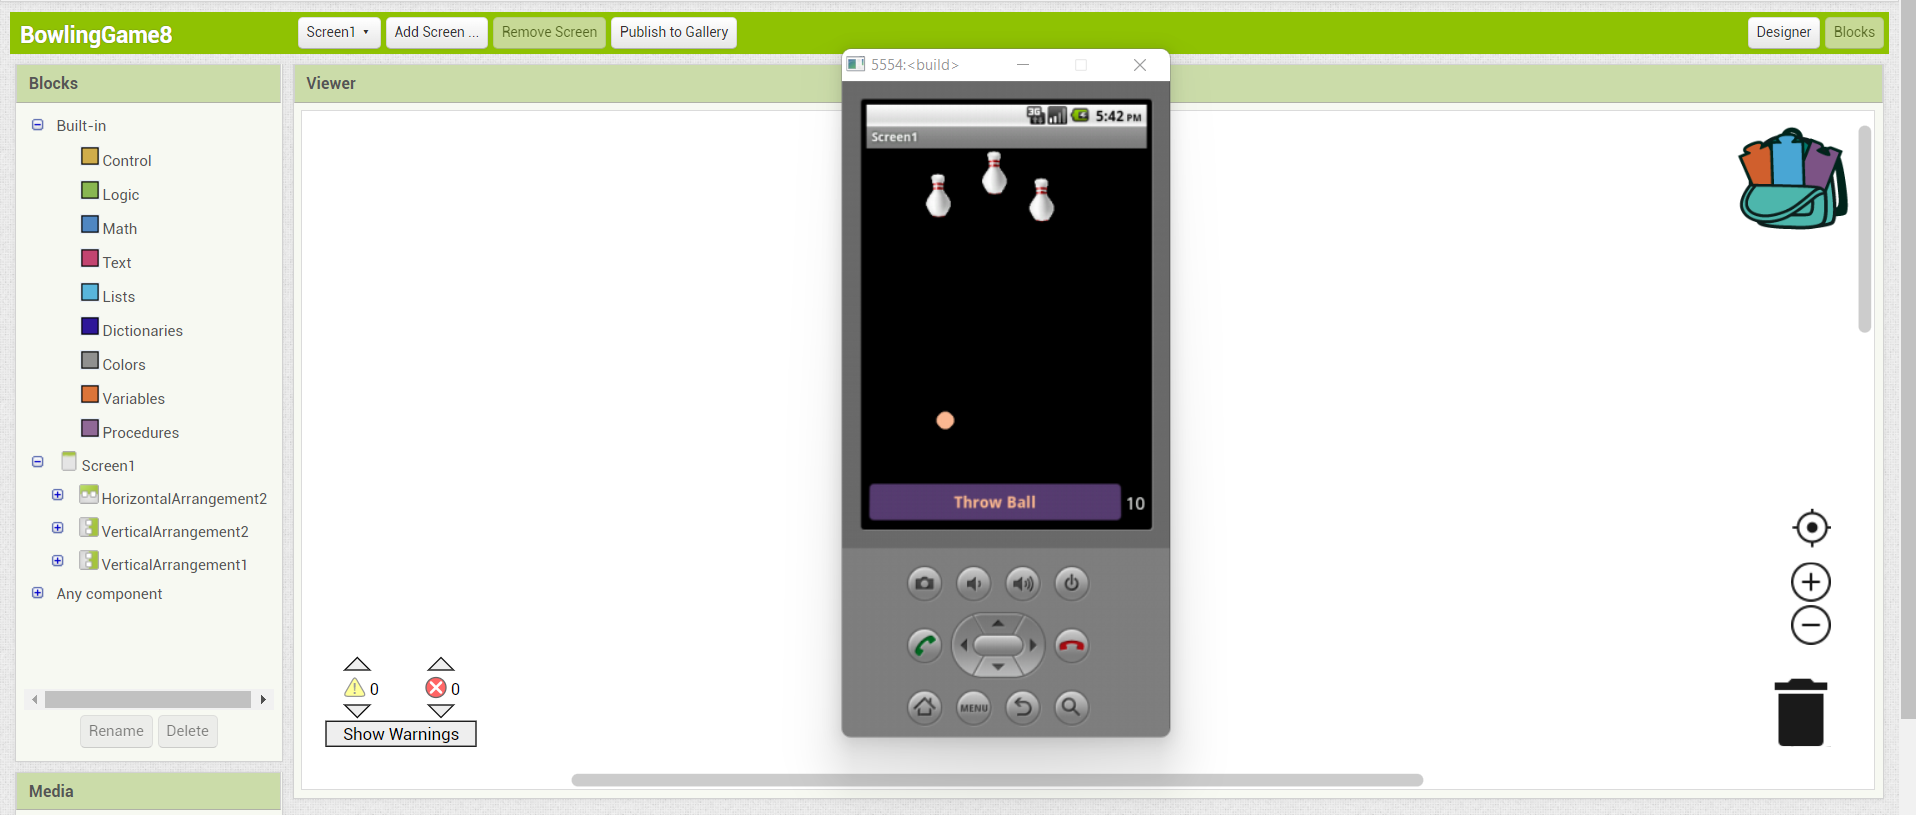
\includegraphics[width=1.0\linewidth,height=0.5\linewidth]{fig130001.png}
  \caption{Боулинг}
\label{fig130001}
\end{figure}

\section{Създаване на дизайна}

В първата стъпка ще създадете началният екран на играта. Върху него ще има един бутон, който ще бъде начало на играта. От групата с елементите Layout трябва да бъде добавен елемента VerticalArrangement. Размерите на елемента трябва да бъдат такива, каквито са размерите на екрана. За това свойствата за височина и ширина трябва да се сменят. За фон на играта освен готовите цветове, може да създадете и свой цвят.

\begin{figure}[H]
  \centering
  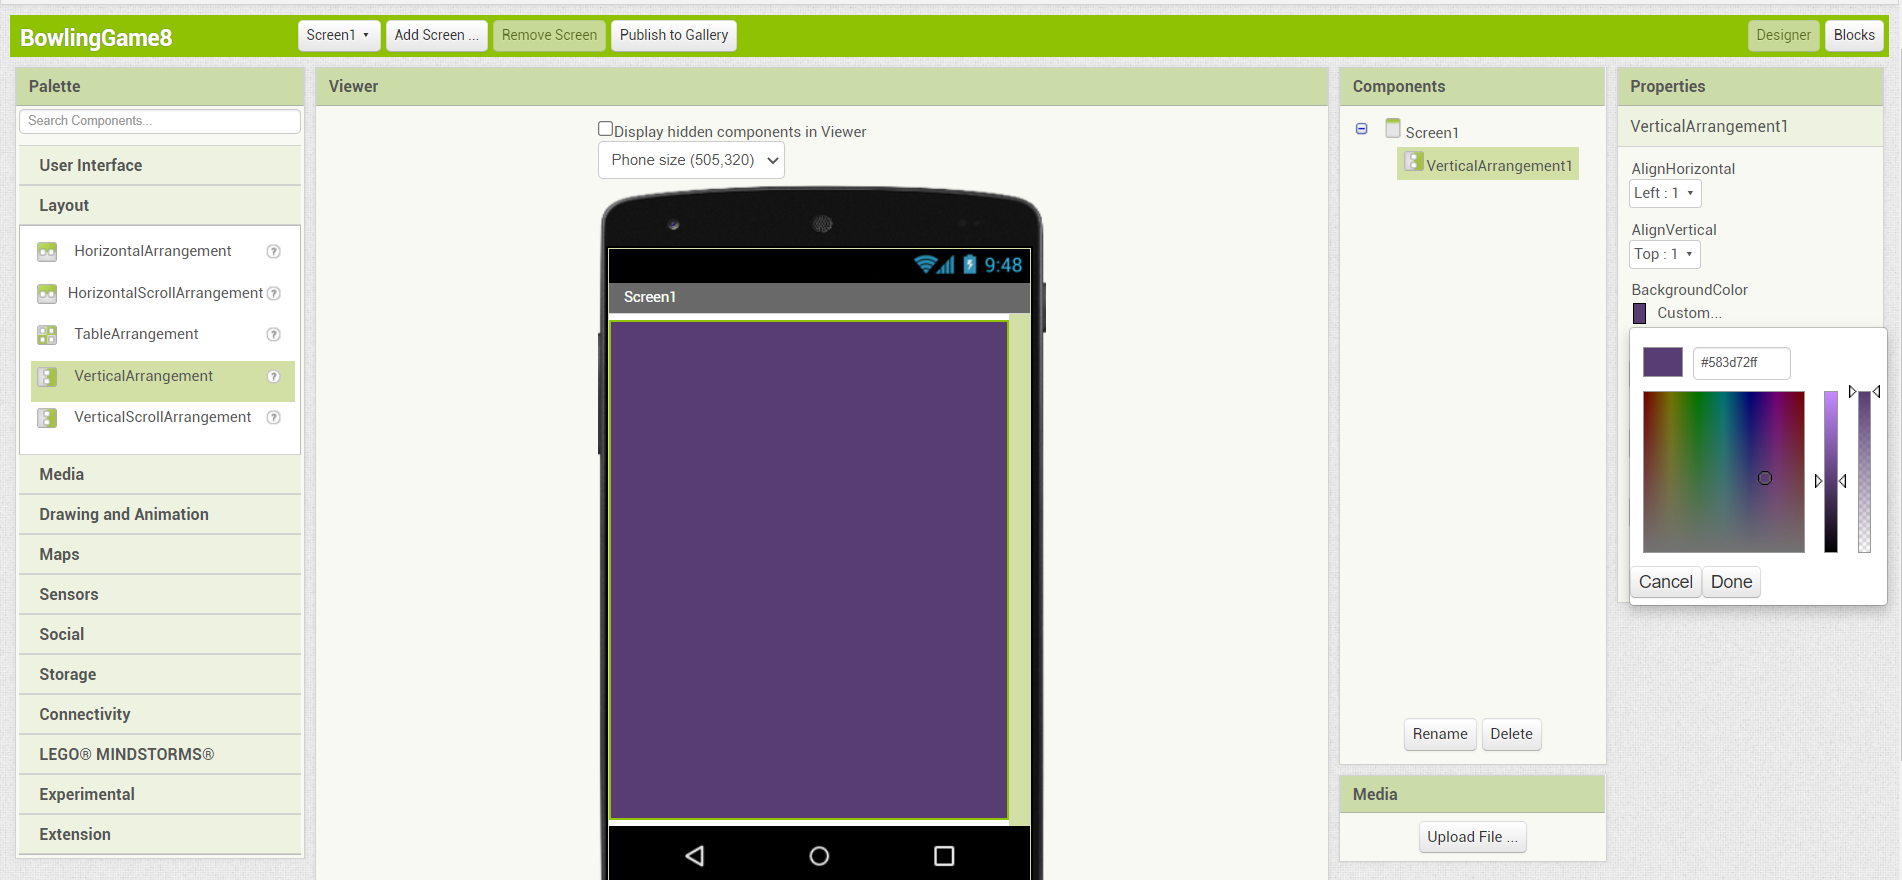
\includegraphics[width=1.0\linewidth,height=0.5\linewidth]{fig130002.png}
  \caption{Начален екран}
\label{fig130002}
\end{figure}

Следва да добавите и бутон за начало на играта. Променете дизайна на бутона и го позиционирайте в средата на екрана.

\begin{figure}[H]
  \centering
  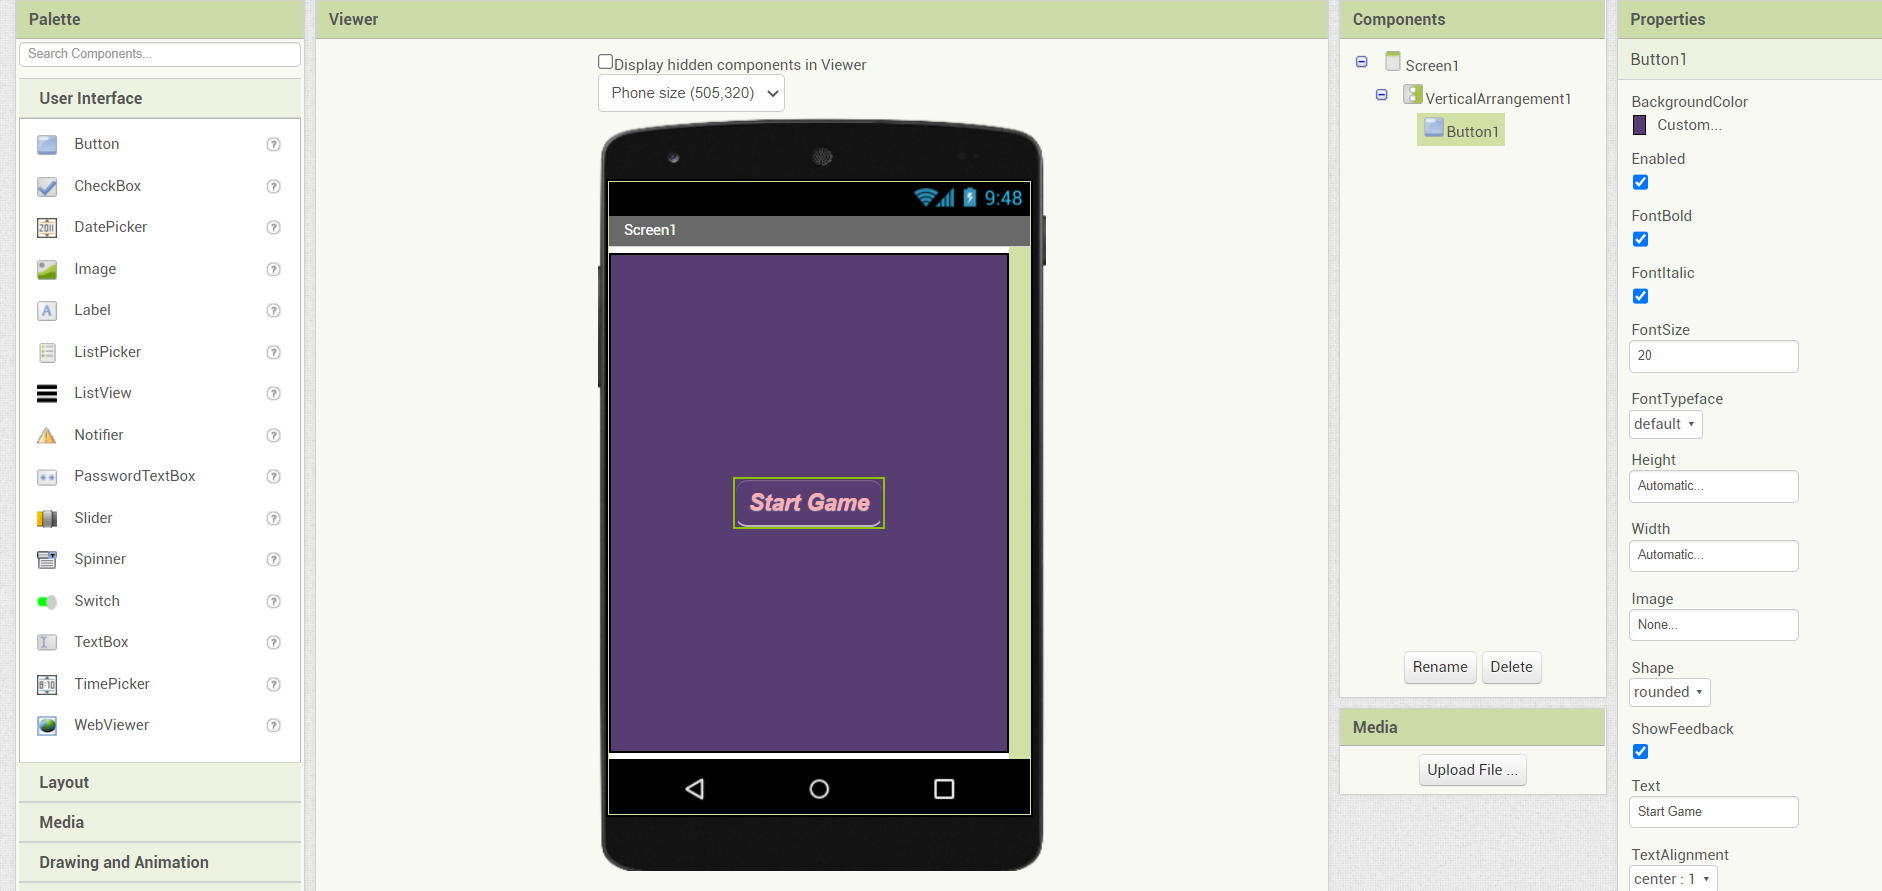
\includegraphics[width=1.0\linewidth,height=0.5\linewidth]{fig130003.png}
  \caption{Бутон за начало на играта}
\label{fig130003}
\end{figure}

В следващата стъпка ще създадете екранът за край на играта. Върху него ще има един бутон за стартиране отново на играта. Също така ще трябва да добавите и надпис, че играта е приключила. Първо от Layout добавете елемент VerticalArrangment. Размерите на елемента трябва да бъдат отново, такива каквито са на екрана. Изберете и подходящ цвят за фон на този екран.

\begin{figure}[H]
  \centering
  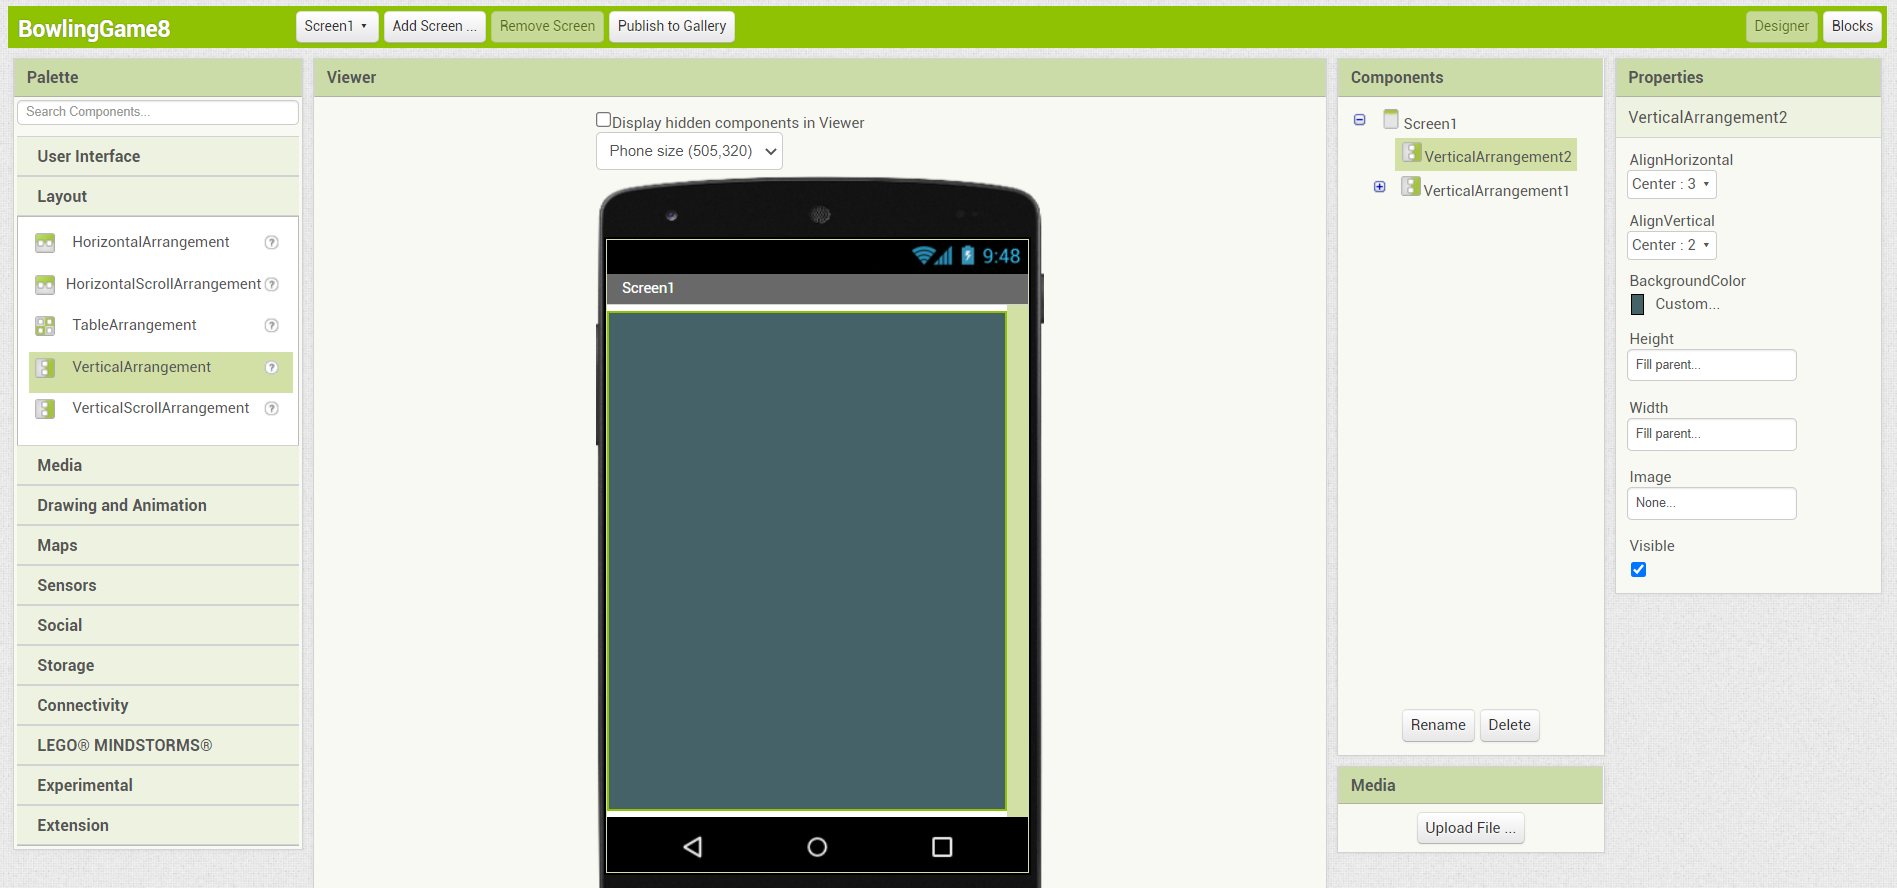
\includegraphics[width=1.0\linewidth,height=0.5\linewidth]{fig130004.png}
  \caption{Краен екран}
\label{fig130004}
\end{figure}

Добавете бутона за започване на играта отново. Променете дизайна му и го позиционирайте в средата на екрана.

\begin{figure}[H]
  \centering
  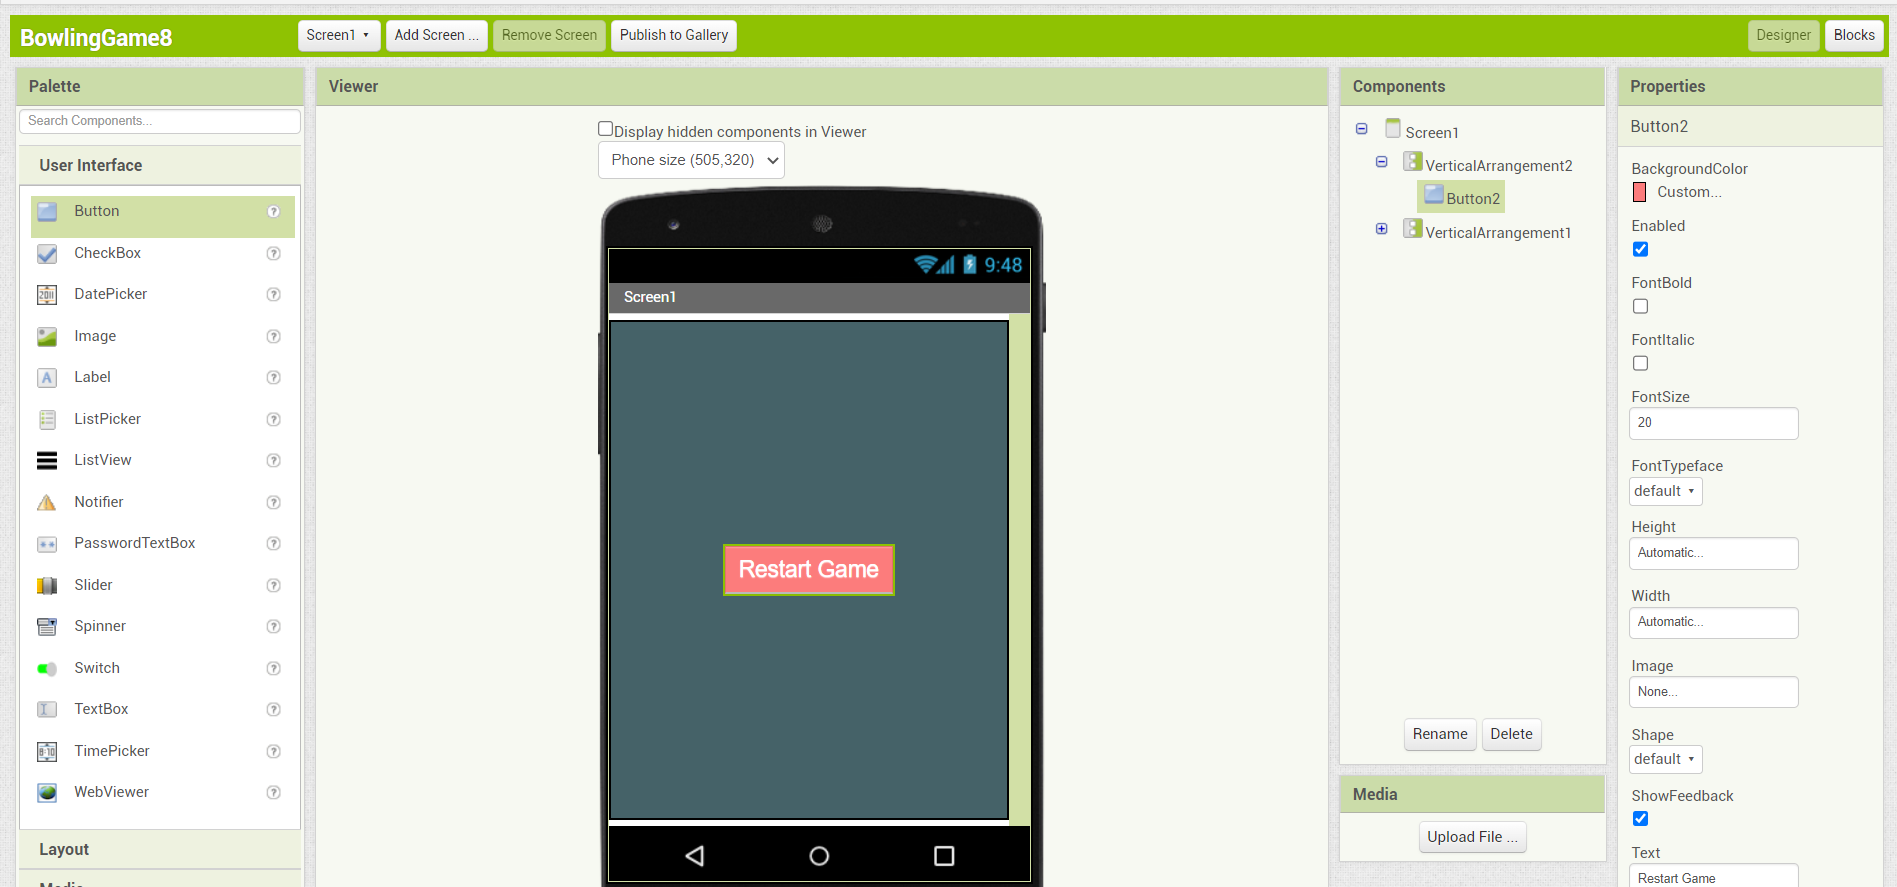
\includegraphics[width=1.0\linewidth,height=0.5\linewidth]{fig130005.png}
  \caption{Бутон за начало на играта отново}
\label{fig130005}
\end{figure}

Добавете и елемент Lable, който да казва Game Over.

\begin{figure}[H]
  \centering
  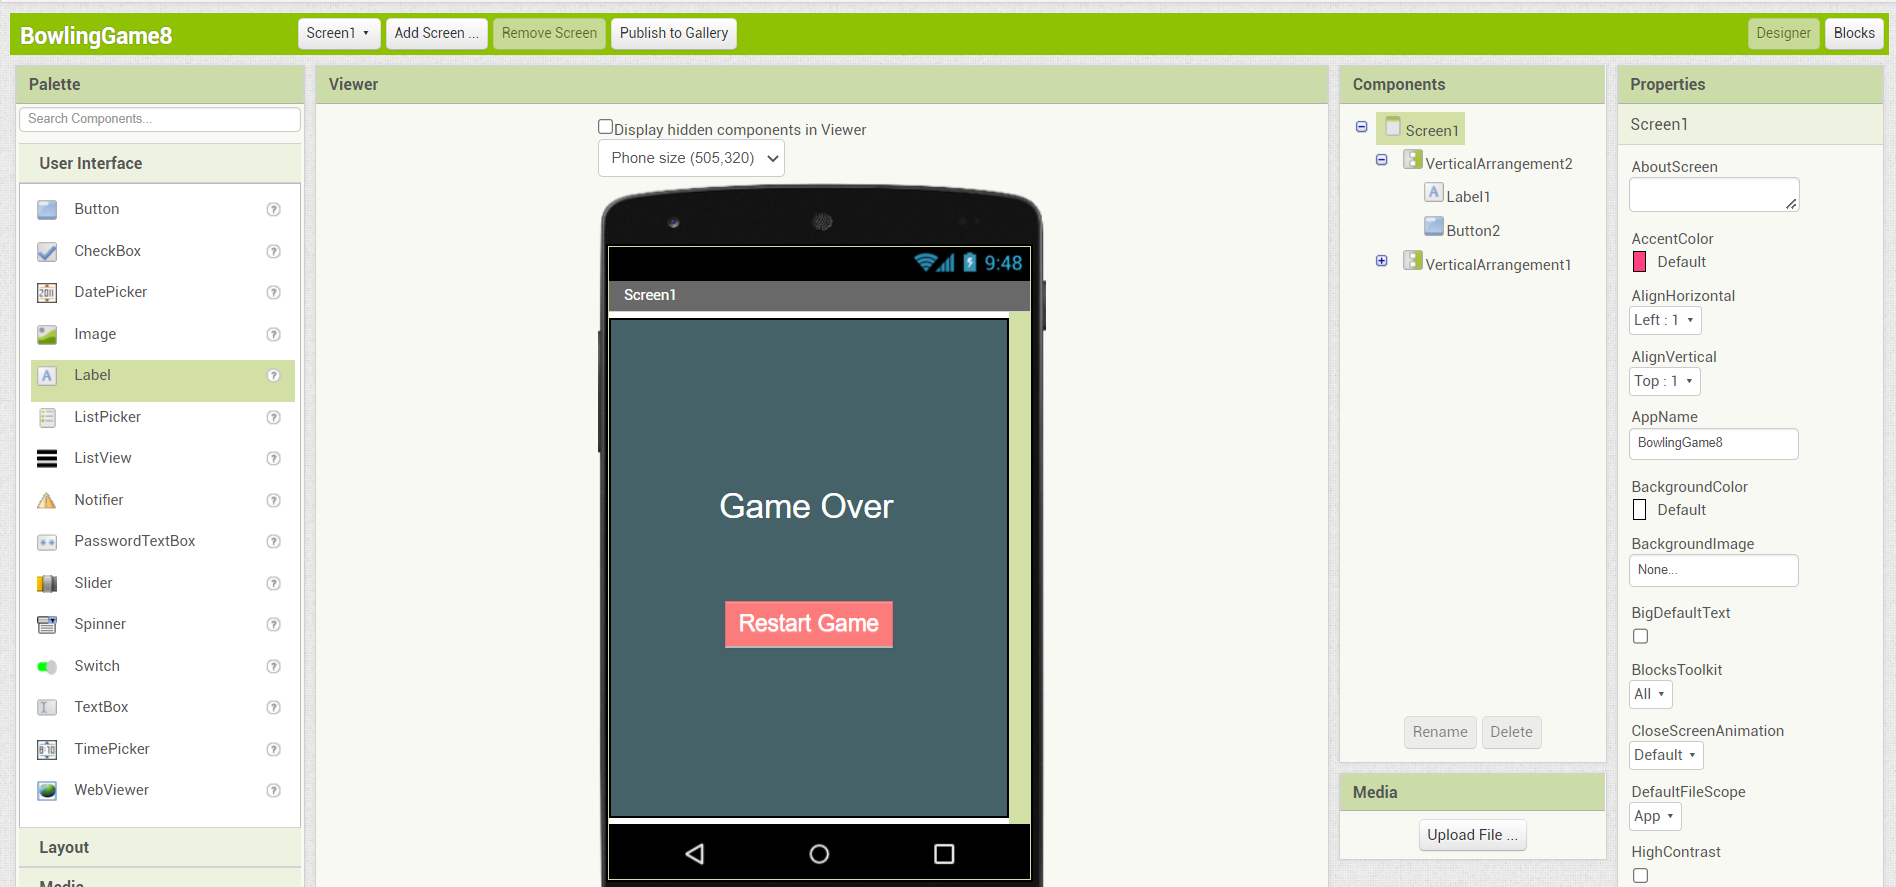
\includegraphics[width=1.0\linewidth,height=0.5\linewidth]{fig130006.png}
  \caption{Надпис за край на играта}
\label{fig130006}
\end{figure}

В последната стъпка ще създадете дизайн на играта. Добавете отново елемент VerticalArrangment. Променете размерите на елемента, като височината и ширината трябва да бъдат толкова, колкото са на екрана. Вътре в този елемент добавете елементът Canvas от секция Drawing and Animation. Променете размера на елемента и цвета на фона.

\begin{figure}[H]
  \centering
  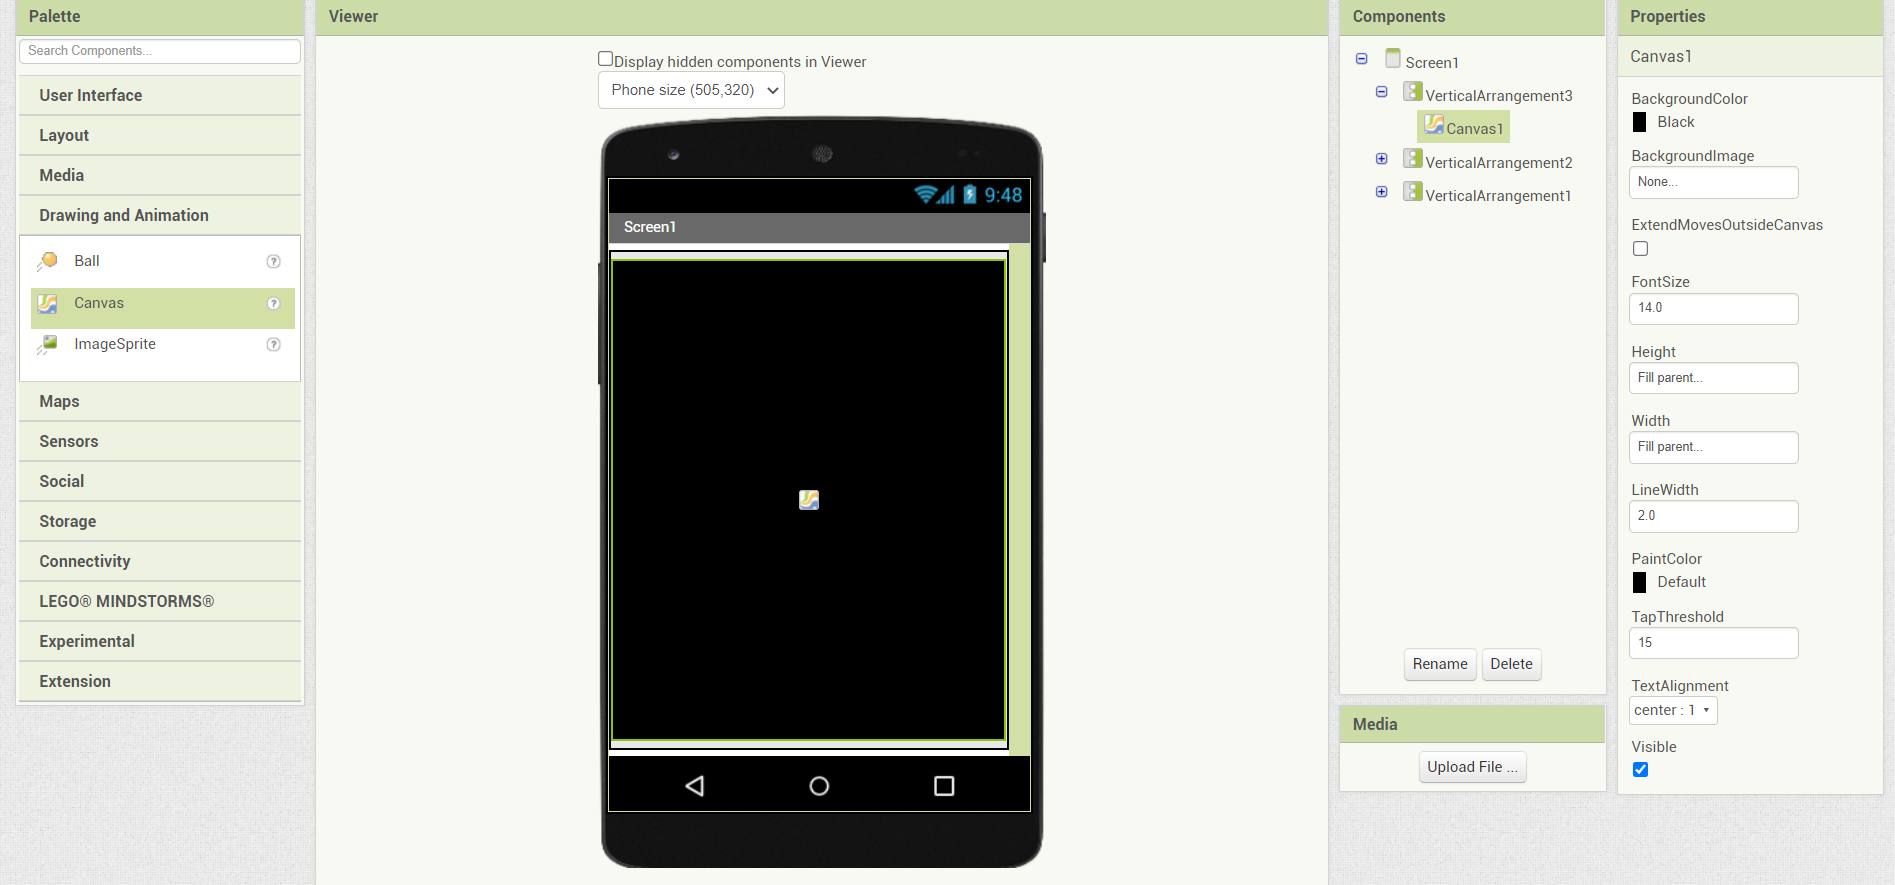
\includegraphics[width=1.0\linewidth,height=0.5\linewidth]{fig130007.png}
  \caption{Екран на играта}
\label{fig130007}
\end{figure}

Добавете елемента топка и променете размерите, позицията и цвета на елемента. Топката трябва да бъде поставена в долната част на екрана.

\begin{figure}[H]
  \centering
  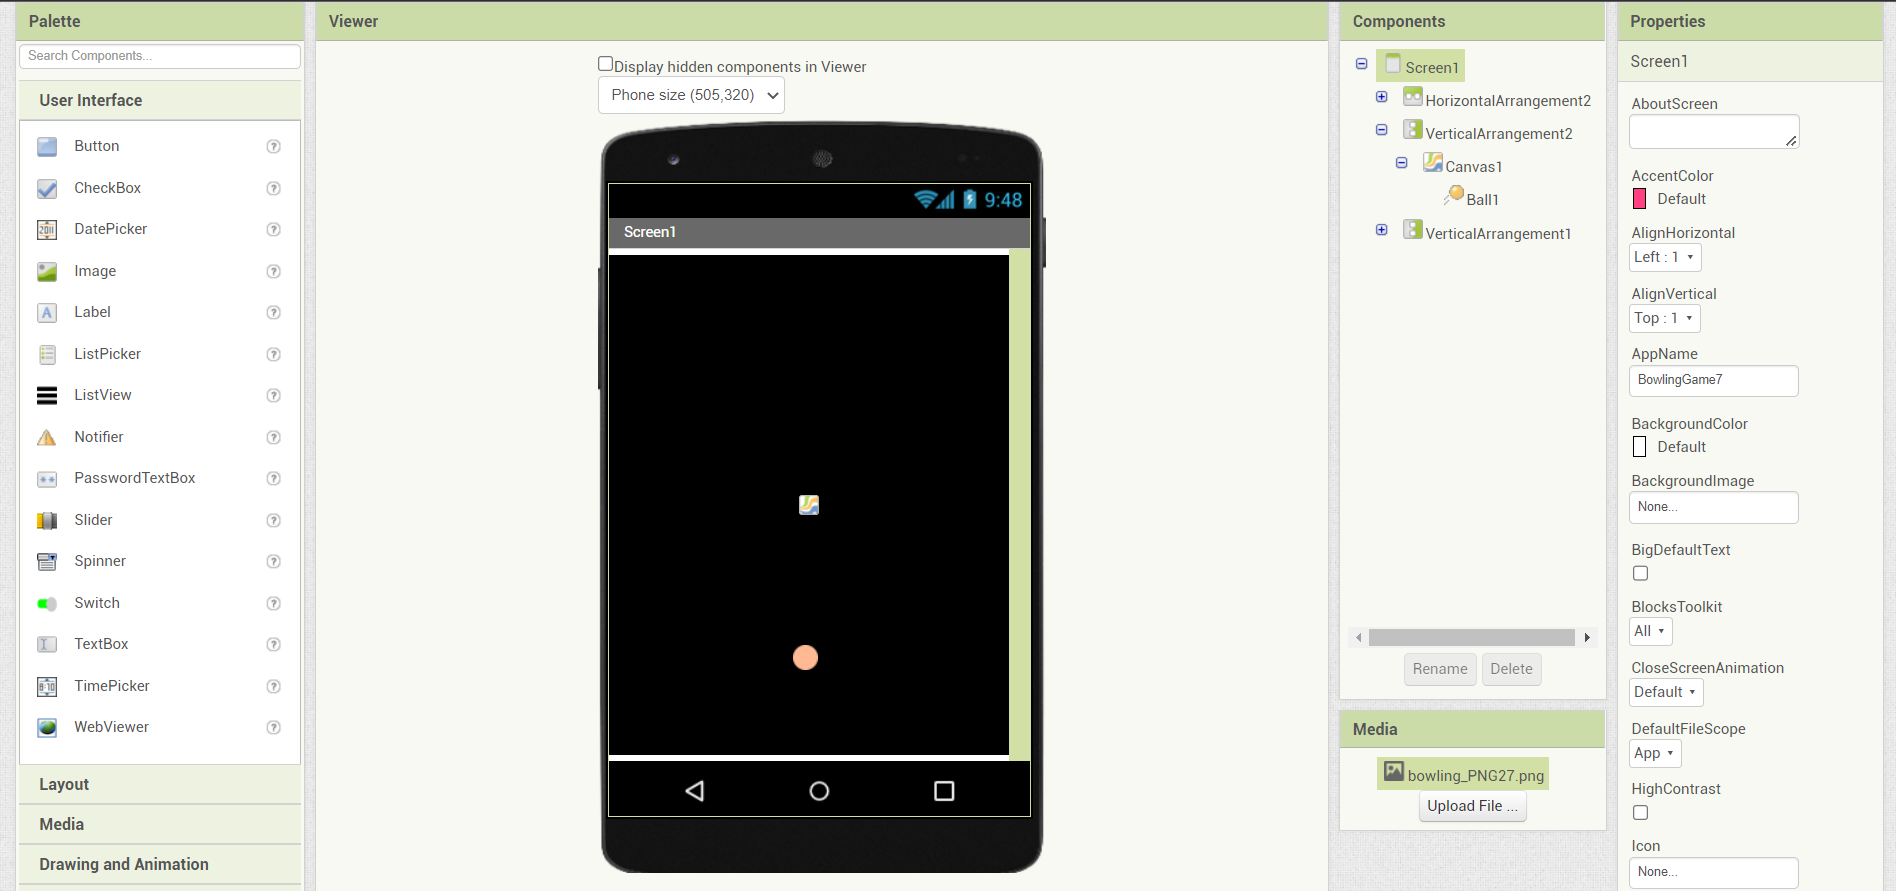
\includegraphics[width=1.0\linewidth,height=0.5\linewidth]{fig130008.png}
  \caption{Добавяне на топката в играта}
\label{fig130008}
\end{figure}

За кеглите може да използвате изображение, което се разпространява със свободен лиценз. Добавете три елемента ImageSprite към елемента Canvas. Към всеки от елементите добавете изображението, което сте изтеглили. Променете размерите и позицията. Трите кегли трбява да се намират в горната част на екрана.

\begin{figure}[H]
  \centering
  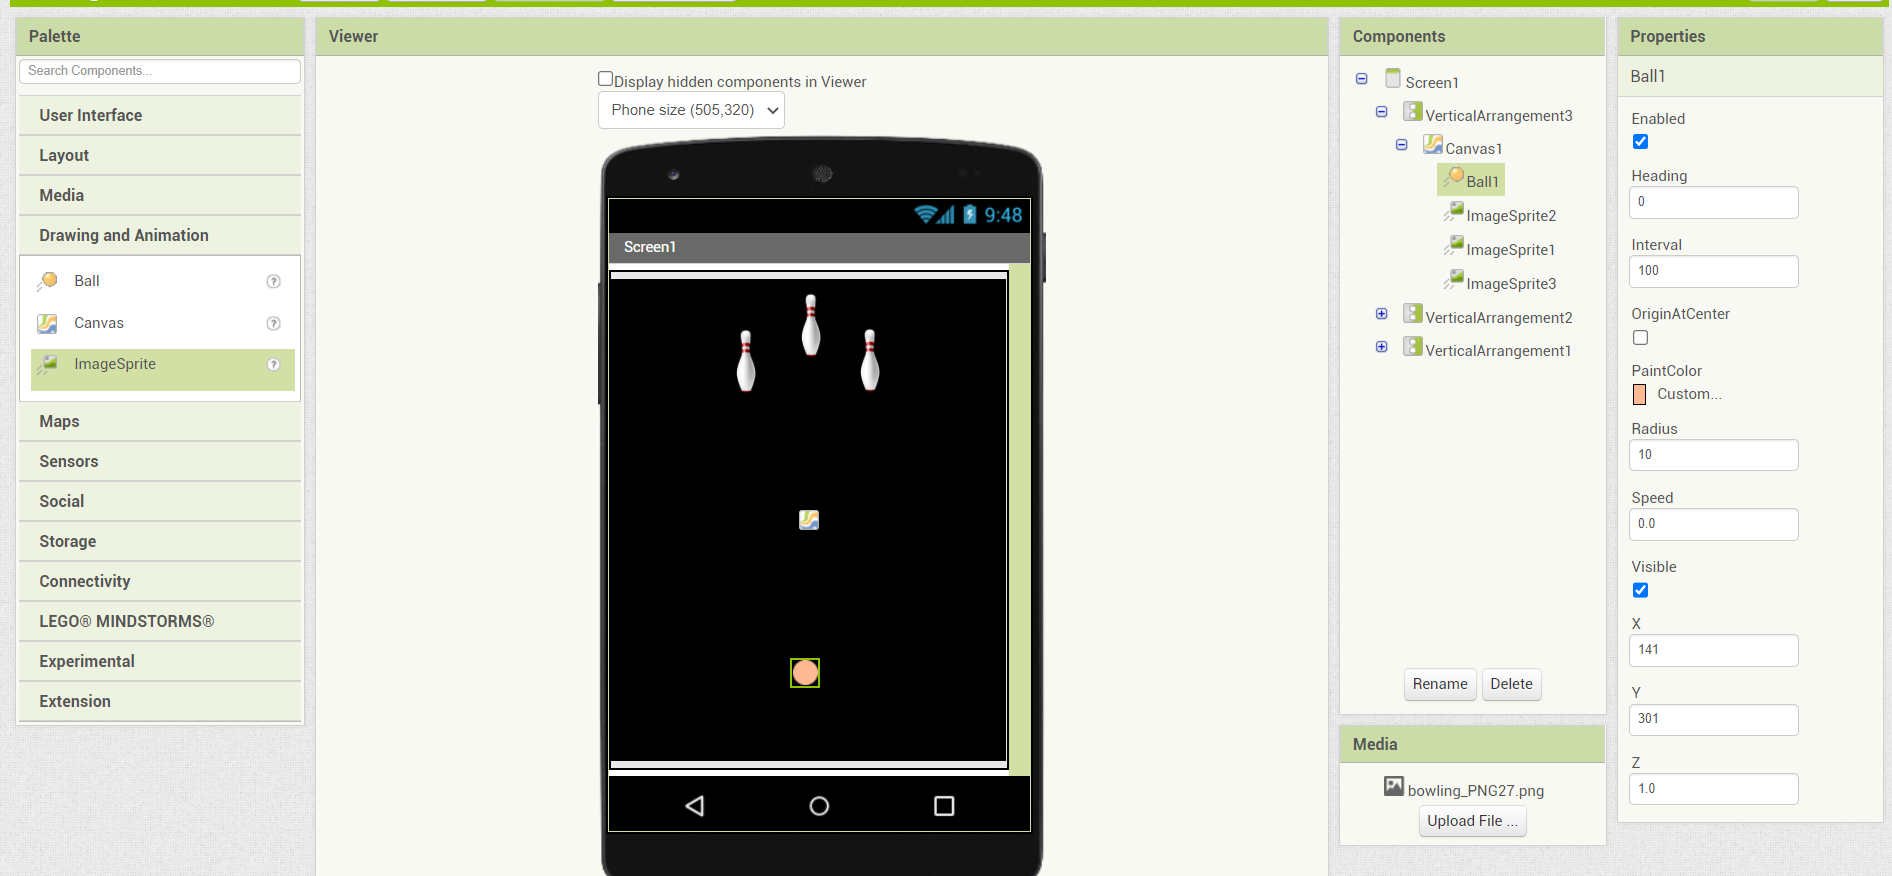
\includegraphics[width=1.0\linewidth,height=0.5\linewidth]{fig130009.png}
  \caption{Добавяне на кеглите}
\label{fig130009}
\end{figure}

В последната част от дизайна трябва да добавите и бутона за изстрелване на топката. Първо добавете елемент HorizontalArrangement. Променете ширината на елемента да бъде толкова, колкото е на екрана.

\begin{figure}[H]
  \centering
  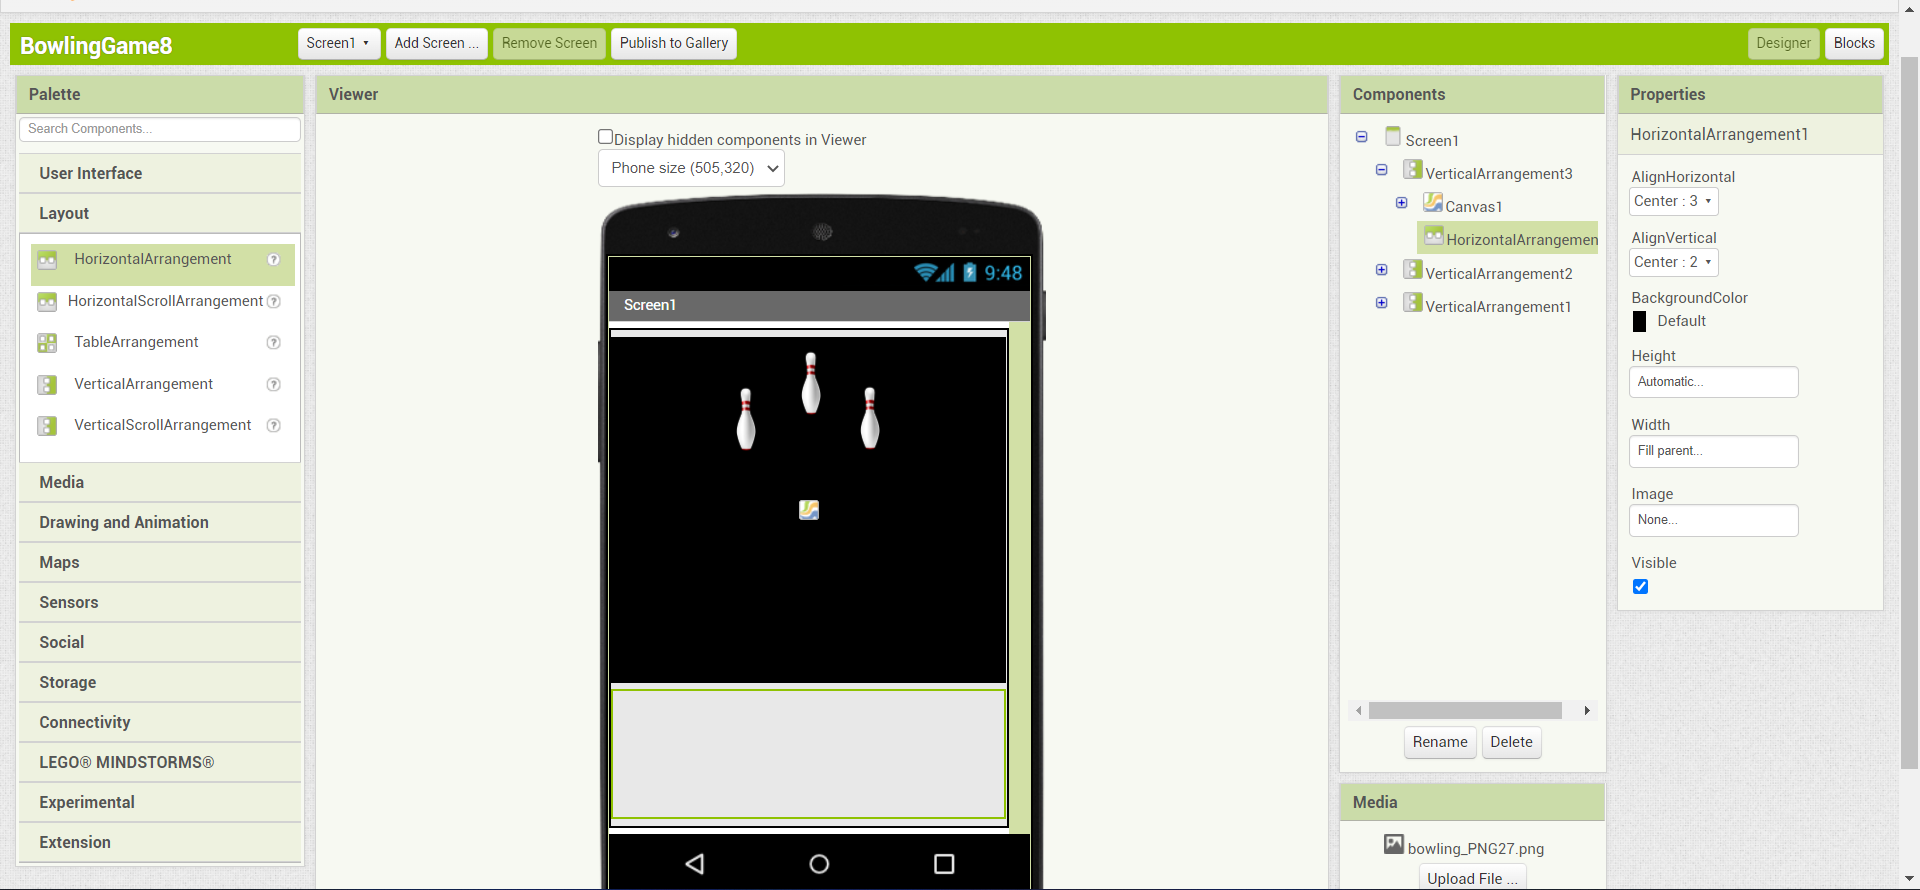
\includegraphics[width=1.0\linewidth,height=0.5\linewidth]{fig130010.png}
  \caption{Добавяне на място за бутона за изстрел}
\label{fig130010}
\end{figure}

Към този елемент добавете още два елемент - бутон и елемент, в който ще за изписва с колко топки разполага героят. Позиционирайте елементите и променете текста на елементите. Може също да промените цвета и формата.

\begin{figure}[H]
  \centering
  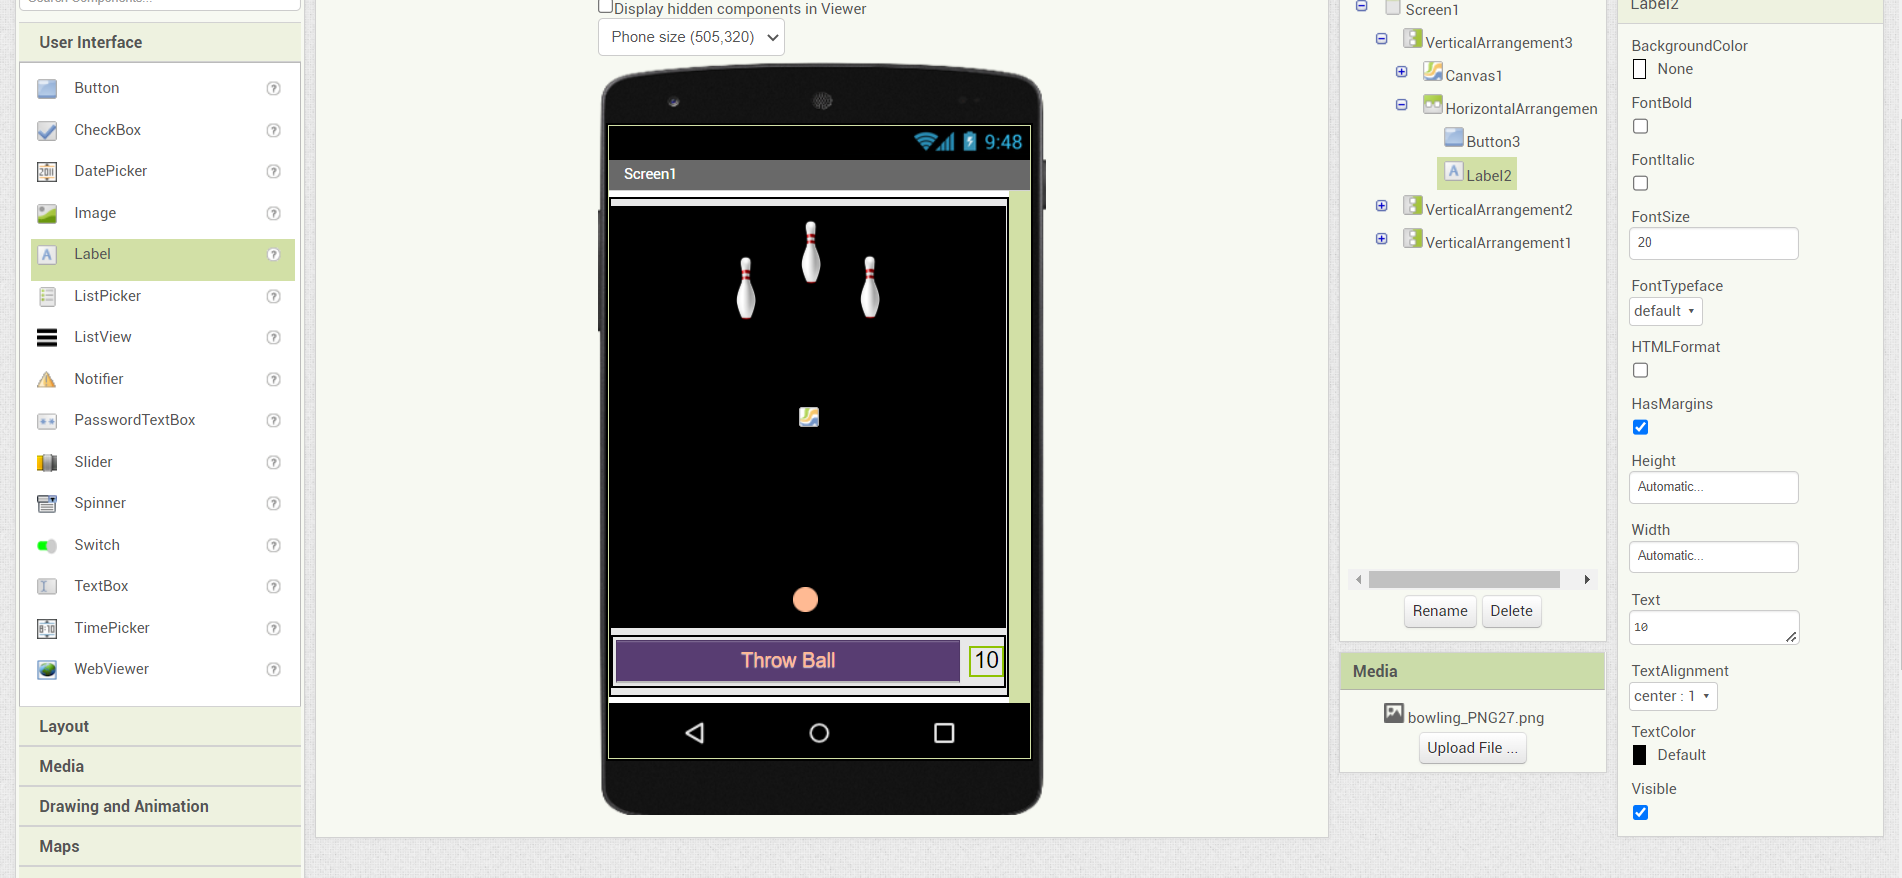
\includegraphics[width=1.0\linewidth,height=0.5\linewidth]{fig130011.png}
  \caption{Добавяне на бутон за изстрел на топката}
\label{fig130011}
\end{figure}

\section{Създаване на програмата}

Преди да започнете да програмирате играта оставете видим само екранът за начало на играта. След това пременете към изгледът за добавяне на блокове.

Започнете с програмирането на бутона за начало на играта. Добавете инструкцията Click, което означава, че когато бутонът е натиснат, тогава ще се изпълнят инструкциите. Когато този бутон бъде настиснат ще задава скорост на топката.

\begin{figure}[H]
  \centering
  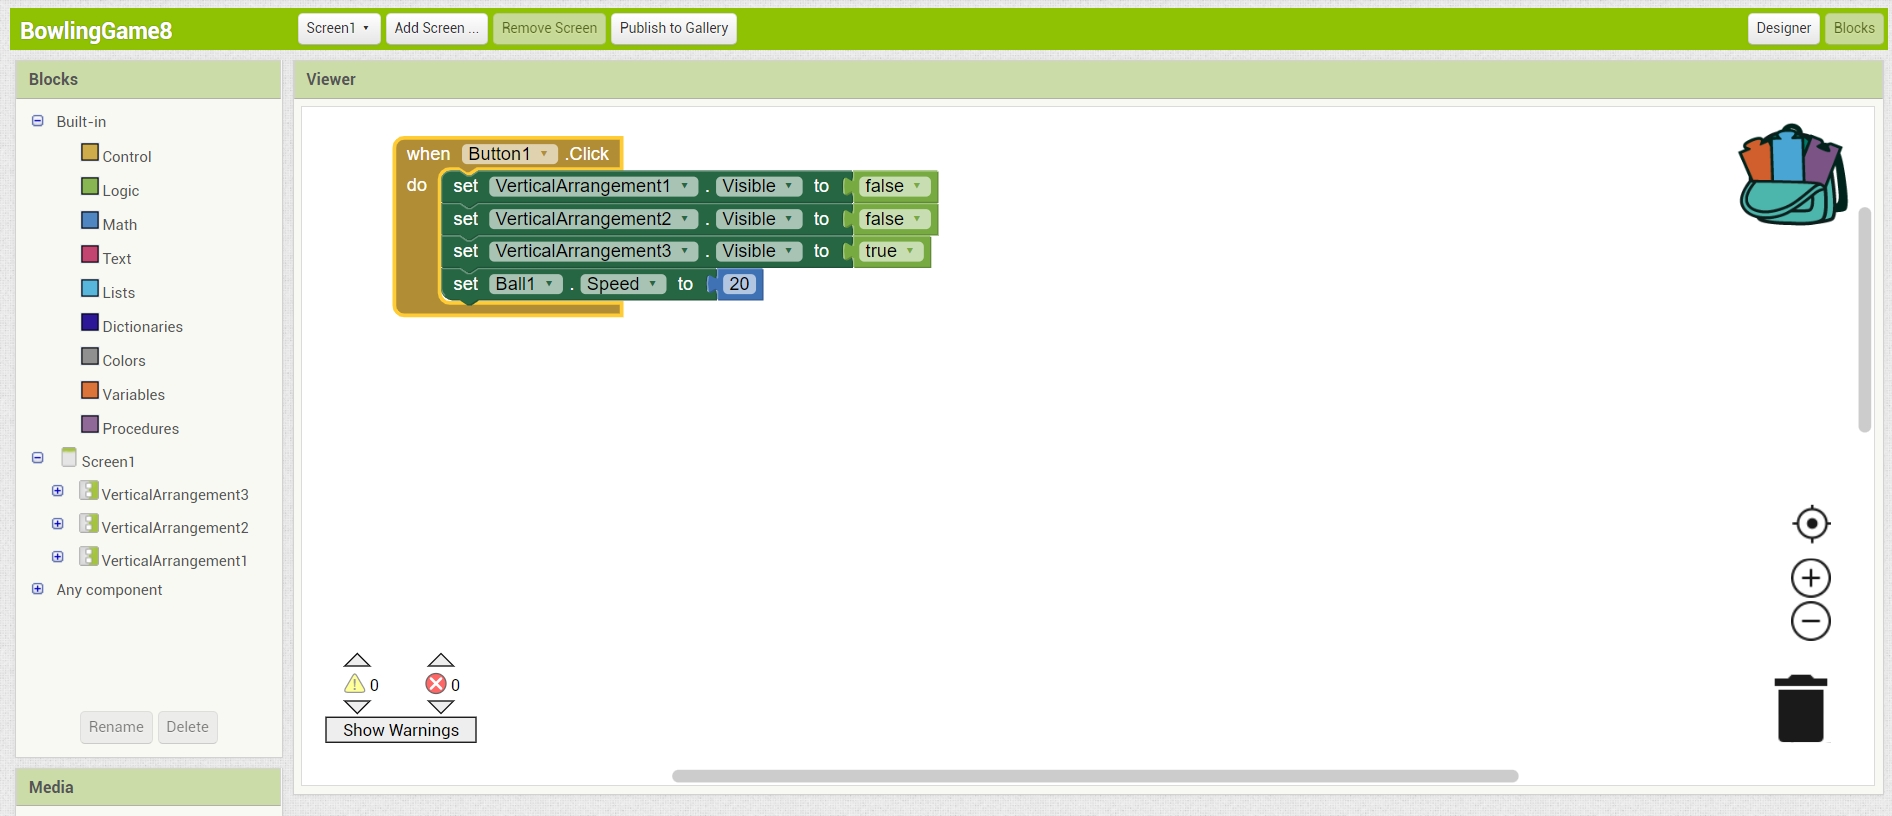
\includegraphics[width=1.0\linewidth,height=0.5\linewidth]{fig130012.png}
  \caption{Инструкции за началния бутон}
\label{fig130012}
\end{figure}

Добавете променлива, която ще е броя на кеглите. Първоначалната стойност нека да бъде 3.

\begin{figure}[H]
  \centering
  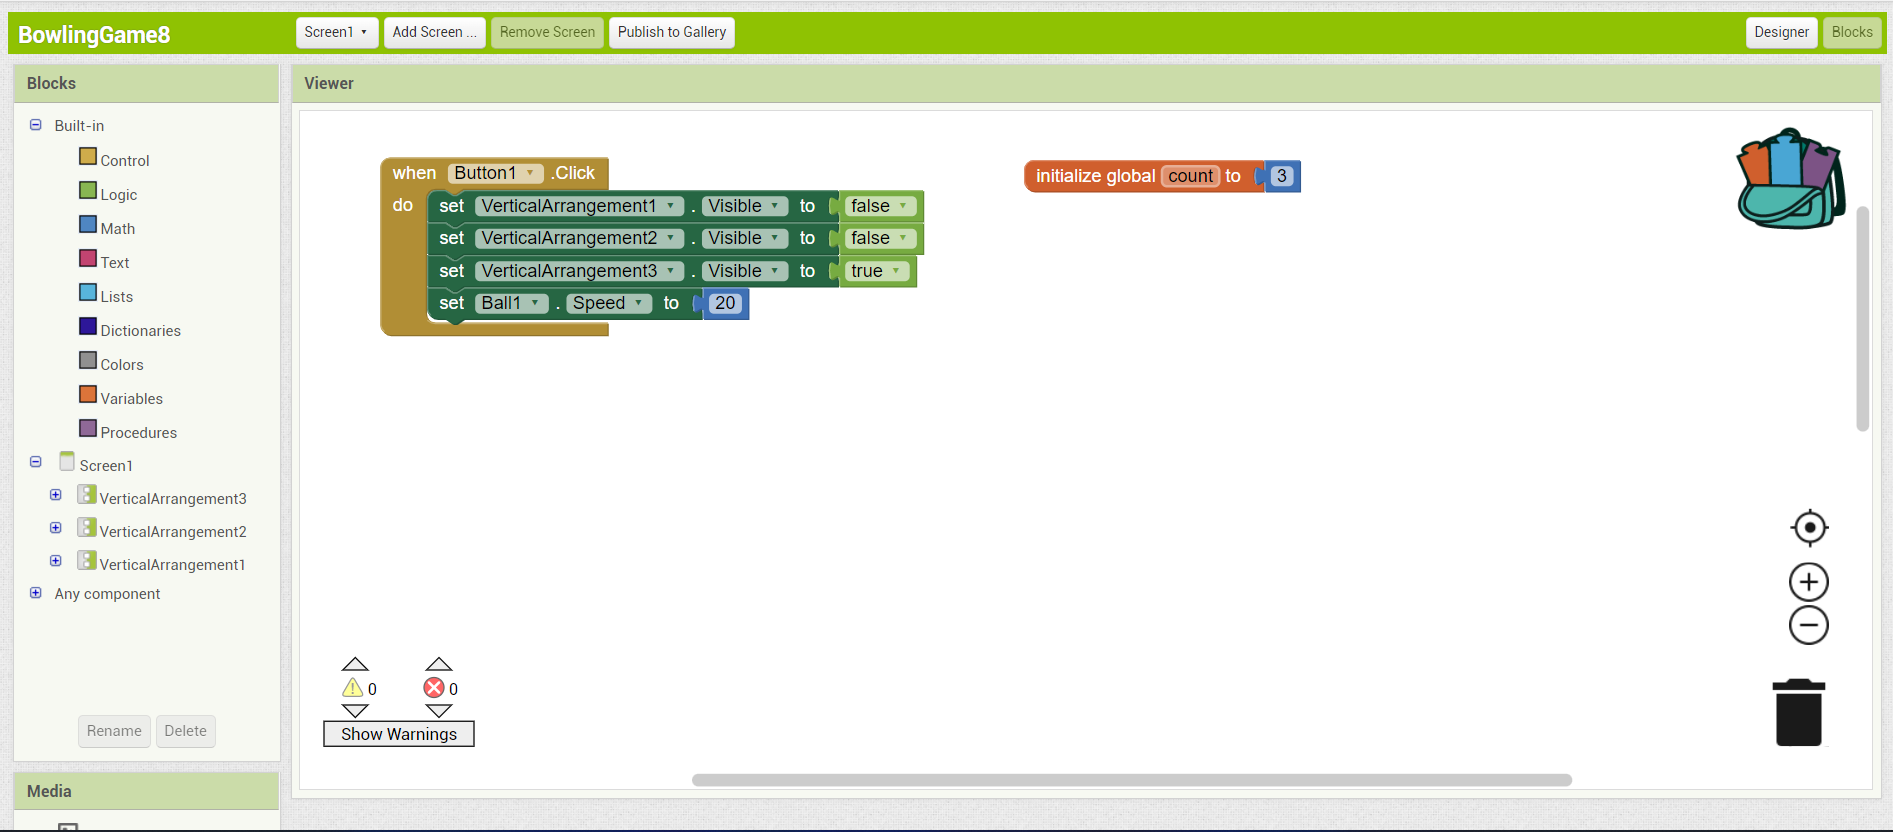
\includegraphics[width=1.0\linewidth,height=0.5\linewidth]{fig130013.png}
  \caption{Променлива за броя кегли}
\label{fig130013}
\end{figure}

Когато топката доконсе някой от ръбовете тя трябва да се отклони. За да се изпълнят инструкциите за отклоняване на топката, първо трябва да се добави събитие. Вътре в това събитие трябва да се направят следните проверки:
- ако топката се намира в най- левия край на екран, тя трябва да се движи надясно
- ако топката се намира в най- десния край на екрана, тя трябва да се движи наляво
- ако топката се намира в най- горния край на екрана, тя трябва да се премести в първоначална позиция.

\begin{figure}[H]
  \centering
  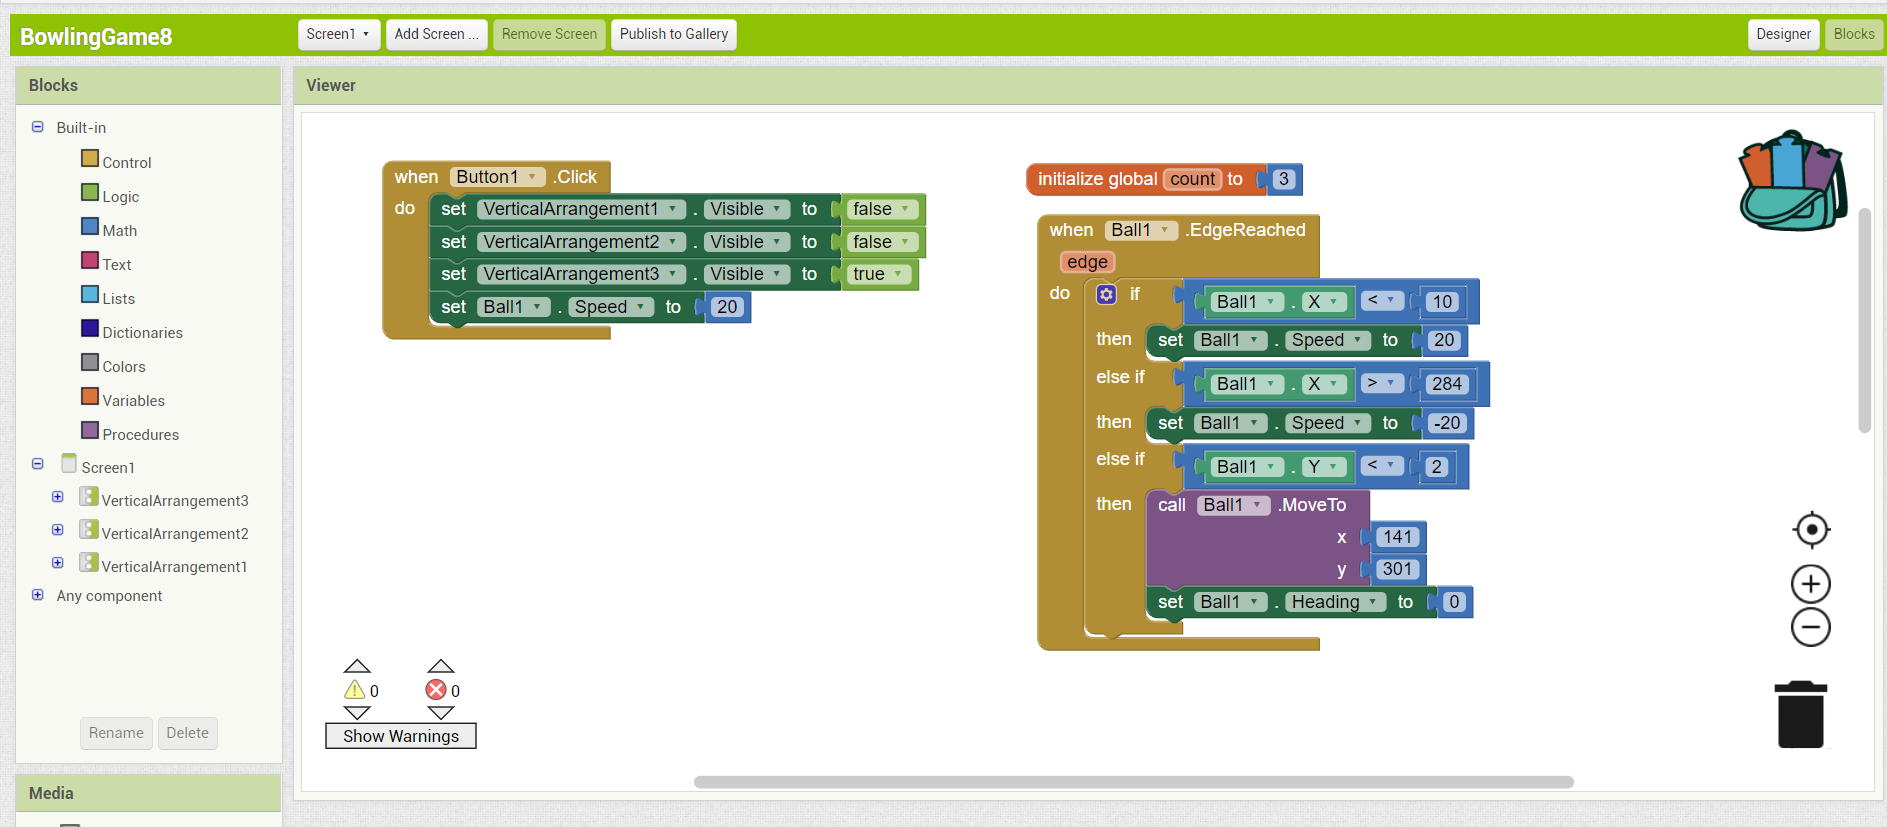
\includegraphics[width=1.0\linewidth,height=0.5\linewidth]{fig130014.png}
  \caption{Движение на топката когато докосне ръб на екрана}
\label{fig130014}
\end{figure}

Другото събитие, което се отнася за топката е, когато тя докосне нещо различно от екрана. В тази игра това може да бъде единствено кегла. Тогава трябва да се промени броя на кеглите, като се извади едно. Друго важно нещо, което трябва да се направи е да се провери дали има още кегли на екрана. Ако няма, то тогава трябва да се скрие този екран и да се покаже последния екран. Важно е да се промени съобщението да изписва Winner.

Ако броя на кеглите не е равен на 0, то тогава трябва да се добави проверка коя кегла е докоснала топката. Целта на това е да може да се направи невидима и да не бъде част от играта.

\begin{figure}[H]
  \centering
  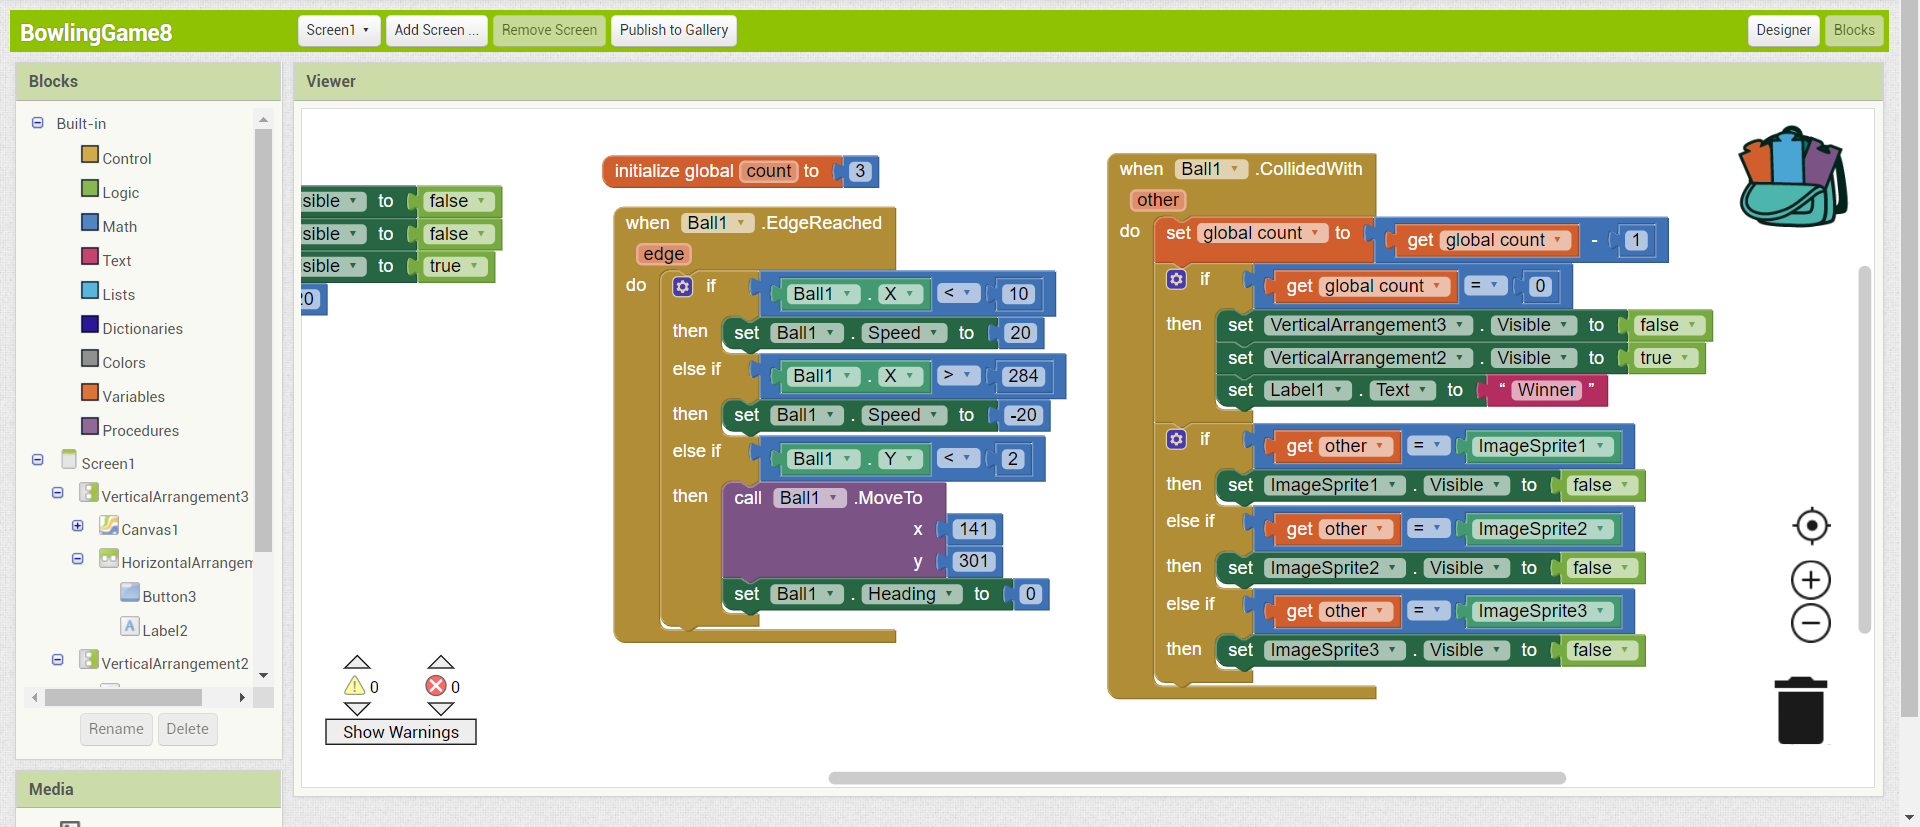
\includegraphics[width=1.0\linewidth,height=0.5\linewidth]{fig130015.png}
  \caption{Инструкции, когато топката докосне кегла}
\label{fig130015}
\end{figure}

Следващите инструкции ще бъдат когато се натисне бутона за изстрелване на топката. Първаа проверка, която трябва да се направи е, ако полето за броя на изстреляните топки е 0, то тогава играта приключва и трябва да се покаже екранът за край на играта. Ако не е равен на 0, то тогава трябва да се зададе посока на топката и да се намали броя с 1.

\begin{figure}[H]
  \centering
  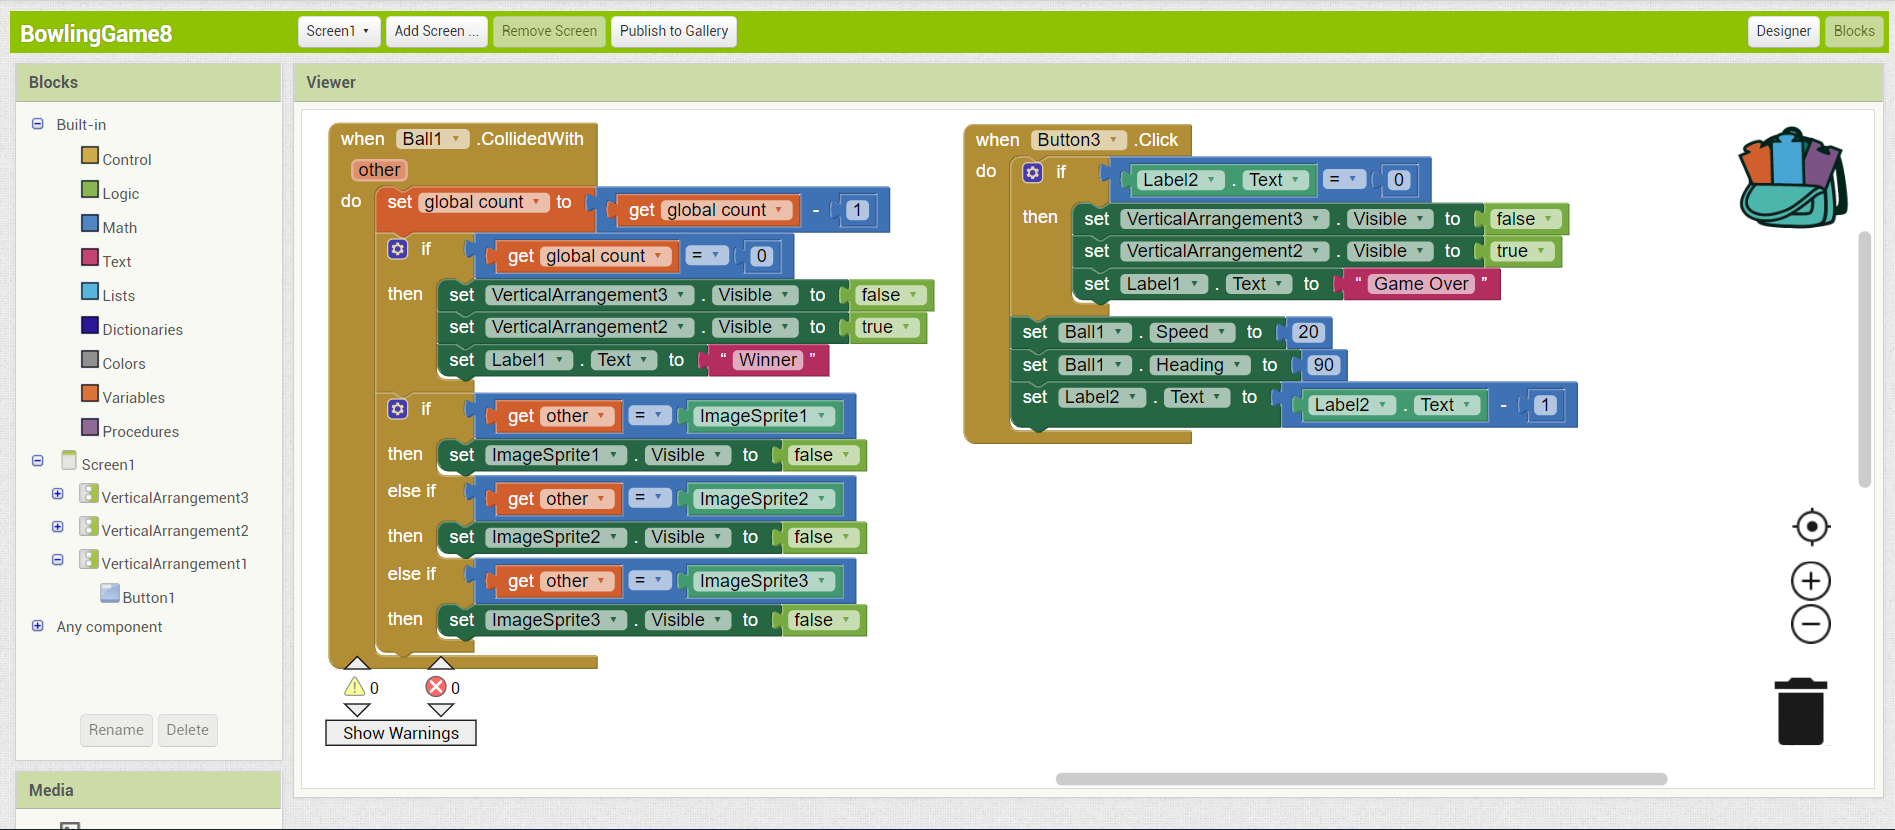
\includegraphics[width=1.0\linewidth,height=0.5\linewidth]{fig130016.png}
  \caption{Инструкции за бутона за изстрел на топката}
\label{fig130016}
\end{figure}

Последните инструкции, които трябва да се добавят са за бутона, който стартира играта от начало. Тези инструкции включват показване на игровия екран, показване на кеглите, задаване на техния брой да бъде 3 и броя на топките да бъде 10.

\begin{figure}[H]
  \centering
  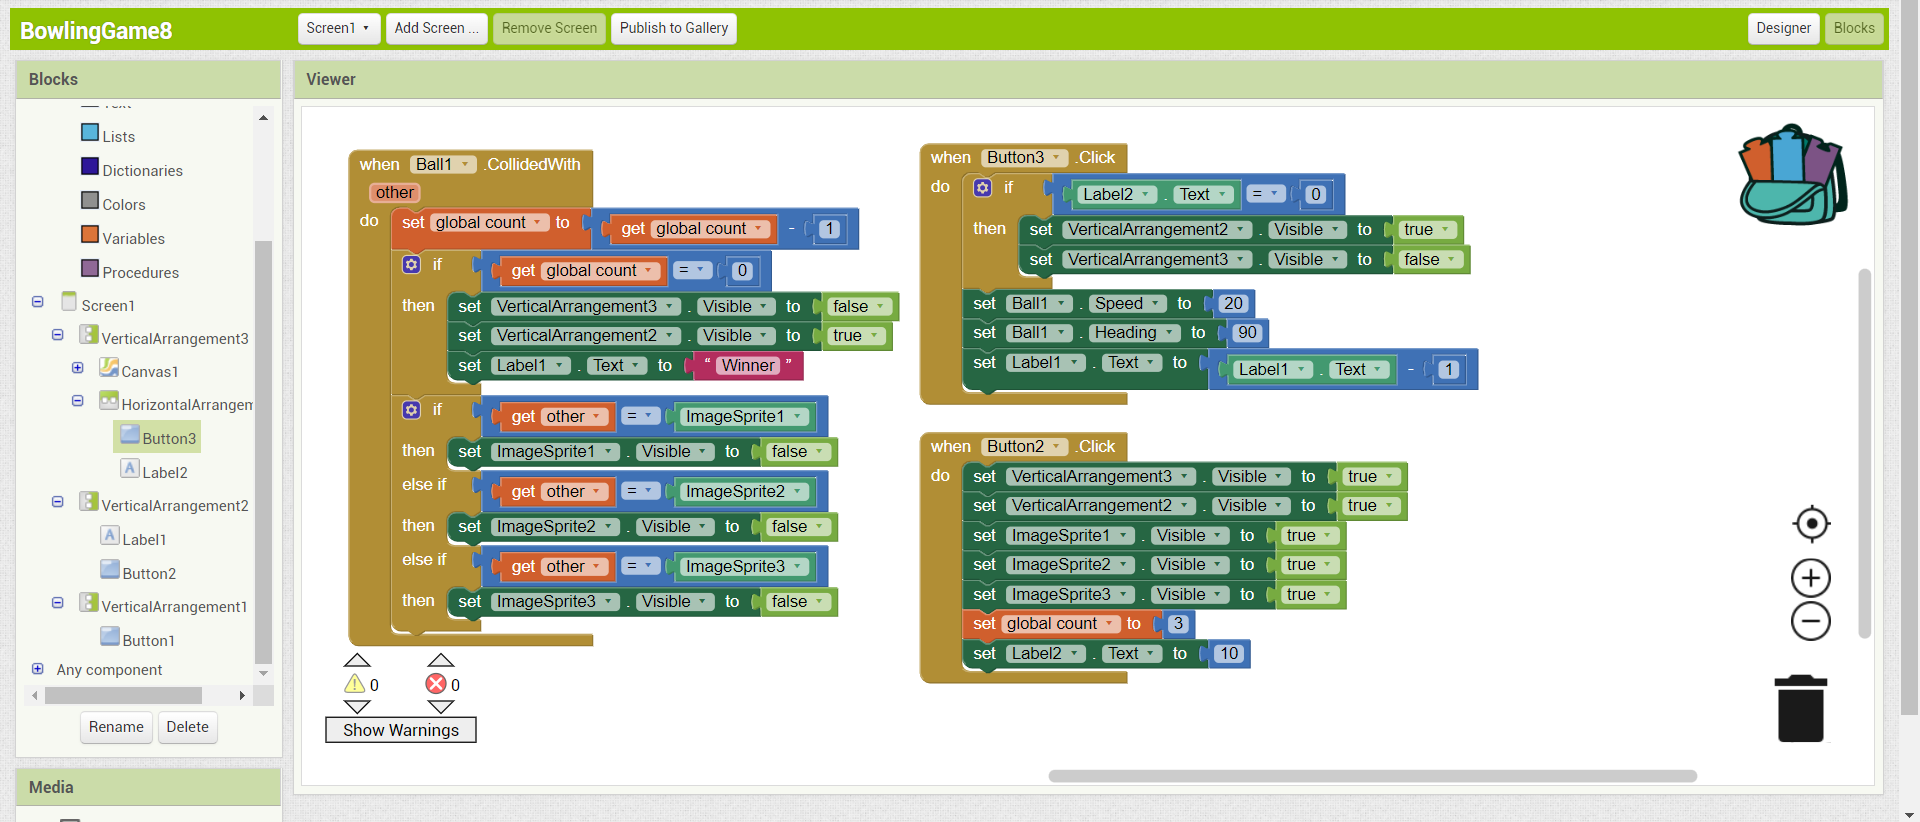
\includegraphics[width=1.0\linewidth,height=0.5\linewidth]{fig130017.png}
  \caption{Инструкции за бутона за започване на играта отначало}
\label{fig130017}
\end{figure}

Пожелаваме ви приятна игра!
